\section{HTTPS}
\subsection{概述}
\ \\
https在http层与TCP连接层之间加入ssl层用于通信内容加密和连接对象身份的认证。其包含如下要求:传输内容加密,即中间节点无法获得双方通信的原始内容,只能获取加密后的结果;消息完整性确认,即传输内容没有被恶意攻击者篡改;身份验证,即连接的服务器确实具有其所声明的身份。一般采用非对称密钥加密技术实现上述要求。每次通讯时服务器向客户端发送其证书以证明其身份。证书通过CA链进行签名,客户端只需逐层验证CA的身份即可证实通讯服务器的身份。openssl库实现了多种加密算法,可以方便地实现创建本地CA、生成非对称密钥、使用CA签名和加密传输等功能。

\subsection{实现}
\ \\
首先使用openssl库生成服务器端的密钥和证书。然后在服务端自建一个CA,使用该CA对服务器端的证书进行签名。由于自建的CA没有经过上层CA链的签名,服务器的身份实际上是不能验证的。

通讯时使用openssl提供的接口进行内容的传输。首先进行加密传输的初始化。通过SSL_read,SSL_write替换原先的read,write函数向客户端收发数据。openssl库使用该函数对发送的报文加密并对收到的报文解密。

\subsection{测试}
\ \\
我们使用openssl实现了https。这时访问服务器可以使用HTTPS协议。初次访问浏览器给出警告,如图\ref{warning}。这是因为我们自建的CA没有经过上层CA链的签名,无法验证服务器端身份。选择允许访问即可使用之前实现的功能。从浏览器端可以查看服务器证书,如图\ref{certificate},和对该证书进行签名的自建CA,如图\ref{ca}。
\begin{figure}
\begin{center}
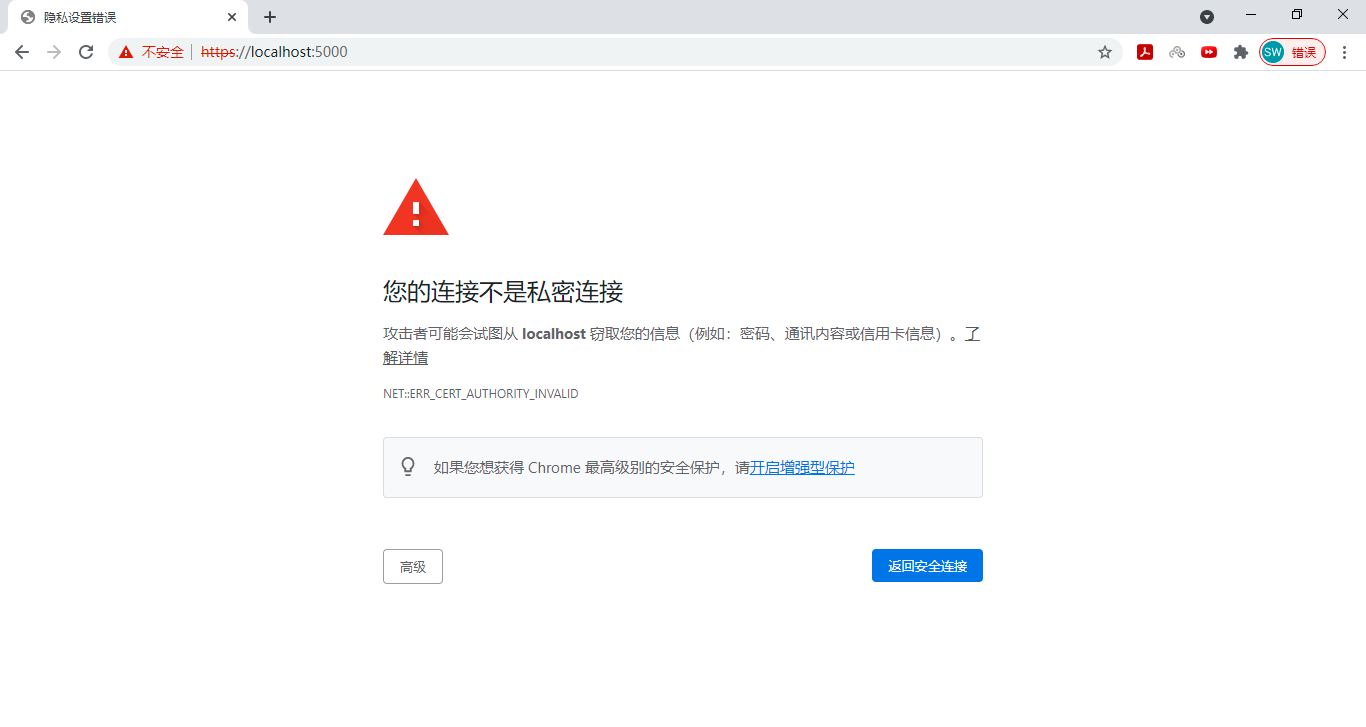
\includegraphics[width=\textwidth]{figs/warning.PNG}
\end{center}
\caption{浏览器警告}
\label{warning}
\end{figure}

\begin{figure}
\begin{center}
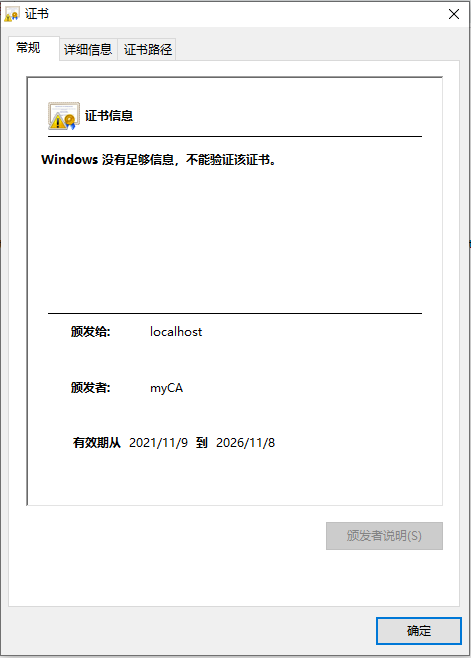
\includegraphics{figs/certificate.PNG}
\end{center}
\caption{证书}
\label{certificate}
\end{figure}

\begin{figure}
\begin{center}
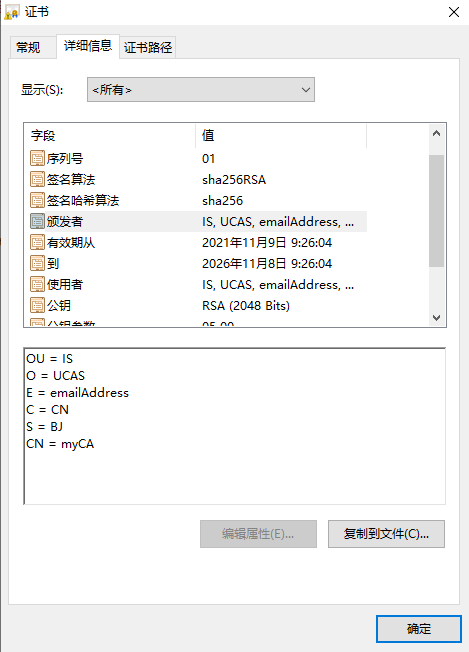
\includegraphics{figs/certificate2.PNG}
\end{center}
\caption{CA}
\label{ca}
\end{figure}